\documentclass[11pt,magyar,a4paper,oneside,]{report}
\usepackage[T1]{fontenc}
\usepackage{ae}
\usepackage{lmodern}
\usepackage{amssymb}
\usepackage{amsmath}
\usepackage{ifxetex,ifluatex}
\usepackage{fixltx2e} % provides \textsubscript
\usepackage{adjustbox}
\usepackage[thmmarks]{ntheorem}
\usepackage{listings}
\usepackage{color}
\usepackage{lastpage}
\usepackage{anysize}
\usepackage{longtable}
\usepackage{sectsty}
\usepackage{setspace}
\usepackage[hang]{caption}
\usepackage{tabularx}
\usepackage{hyphenat}
\usepackage{enumitem}
\usepackage{subcaption}
\usepackage{todonotes}
\usepackage{adjustbox}
\usepackage{minibox}
\usepackage{pdfpages}
\usepackage{tikz}
% fix for pandoc 1.14
\providecommand{\tightlist}{%
  \setlength{\itemsep}{0pt}\setlength{\parskip}{0pt}}
% use microtype if available
\IfFileExists{microtype.sty}{\usepackage{microtype}}{}
% use upquote if available, for straight quotes in verbatim environments
\IfFileExists{upquote.sty}{\usepackage{upquote}}{}
\ifnum 0\ifxetex 1\fi\ifluatex 1\fi=0 % if pdftex
  \usepackage[utf8]{inputenc}
\else % if luatex or xelatex
  \usepackage{fontspec}
  \ifxetex
    \usepackage{xltxtra,xunicode}
  \fi
  \defaultfontfeatures{Mapping=tex-text,Scale=MatchLowercase}
  \newcommand{\euro}{€}
\fi
\usepackage{natbib}
\bibliographystyle{plain}
\usepackage{graphicx}
% We will generate all images so they have a width \maxwidth. This means
% that they will get their normal width if they fit onto the page, but
% are scaled down if they would overflow the margins.
\makeatletter
\def\maxwidth{\ifdim\Gin@nat@width>\linewidth\linewidth
\else\Gin@nat@width\fi}
\makeatother
\let\Oldincludegraphics\includegraphics
%\renewcommand{\includegraphics}[1]{\Oldincludegraphics[scale=1.0]{#1}}
\renewcommand{\includegraphics}[1]{
\begin{adjustbox}{max size={\textwidth}{\textheight}}
    \Oldincludegraphics[scale=0.6]{#1}%
\end{adjustbox}
}
\ifxetex
  \usepackage[setpagesize=false, % page size defined by xetex
              unicode=false, % unicode breaks when used with xetex
              xetex]{hyperref}
\else
  \usepackage[unicode=true]{hyperref}
\fi
\definecolor{darkgreen}{rgb}{0,0.5,0}
\hypersetup{breaklinks=true,
            bookmarks=true,
            pdfauthor={},
            pdftitle={},
            colorlinks=true,
            urlcolor=blue,
            linkcolor=magenta,
            citecolor=darkgreen,
            pdfborder={0 0 0}}
\urlstyle{same}  % don't use monospace font for urls
\setlength{\parindent}{0pt}
\setlength{\parskip}{6pt plus 2pt minus 1pt}
\setlength{\emergencystretch}{3em}  % prevent overfull lines
\ifxetex
  \usepackage{polyglossia}
  \setmainlanguage{}
\else
  \usepackage[magyar]{babel}
\fi

\title{Mikroszolgáltatásokra épülő architektúra fejlesztésének és tesztelésének támogatása}
\author{Borlay Dániel}

\renewcommand*{\hyperref}[2][\ar]{%
  \def\ar{#2}
  #2 (\refstruc{#1})}

\renewcommand*{\figureautorefname}{ábra}

\sloppy

% for English documents
%\setlength{\parindent}{0pt} % áttekinthetőbb, angol nyelvű dokumentumokban jellemző
%\setlength{\parskip}{8pt plus 3pt minus 3pt} % áttekinthetőbb, angol nyelvű dokumentumokban jellemző

% for Hungarian documents
\setlength{\parindent}{12pt}
\setlength{\parskip}{0pt}

\marginsize{35mm}{25mm}{15mm}{15mm} % anysize package
\setcounter{secnumdepth}{0}
\sectionfont{\large\upshape\bfseries}
\setcounter{secnumdepth}{3}
\singlespacing
\frenchspacing


\begin{document}

\footnotesize


\normalsize

%--------------------------------------------------------------------------------------
% The title page
%--------------------------------------------------------------------------------------
\begin{titlepage}
\begin{center}
\Oldincludegraphics[width=60mm,keepaspectratio]{img/BME1782logo.pdf}\\

\vspace{0.3cm}
\textbf{Budapesti Műszaki és Gazdaságtudományi Egyetem}\\
\textmd{Méréstechnika és Információs Rendszerek Tanszék}\\
\textmd{}\\[5cm]

\vspace{0.4cm}
{\huge \bfseries Mikroszolgáltatásokra épülő architektúra fejlesztésének és tesztelésének támogatása}\\[0.8cm]
\vspace{0.5cm}
\textsc{\Large Diplomaterv}\\[4cm]

\begin{tabular}{cc}
 \makebox[7cm]{\emph{Készítette}} & \makebox[7cm]{\emph{Konzulens}} \\
 \makebox[7cm]{Borlay Dániel} & \makebox[7cm]{Szatmári Zoltán}
\end{tabular}

\vfill
{\large \today}
\end{center}
\end{titlepage}

\onehalfspacing

\hypersetup{linkcolor=black}
\setcounter{tocdepth}{2}
\tableofcontents

\vfill
\clearpage

\begin{center}
\large
\textbf{HALLGATÓI NYILATKOZAT}\\
\end{center}

Alulírott \emph{Borlay Dániel}, szigorló hallgató kijelentem, hogy ezt a diplomatervet meg nem engedett segítség nélkül, saját magam készítettem, csak a megadott forrásokat (szakirodalom, eszközök stb.) használtam fel. Minden olyan részt, melyet szó szerint, vagy azonos értelemben, de átfogalmazva más forrásból átvettem, egyértelműen, a forrás megadásával megjelöltem.

Hozzájárulok, hogy a jelen munkám alapadatait (szerző(k), cím, angol és magyar nyelvű tartalmi kivonat, készítés éve, konzulens(ek) neve) a BME VIK nyilvánosan hozzáférhető elektronikus formában, a munka teljes szövegét pedig az egyetem belső hálózatán keresztül (vagy autentikált felhasználók számára) közzétegye. Kijelentem, hogy a benyújtott munka és annak elektronikus verziója megegyezik. Dékáni engedéllyel titkosított diplomatervek esetén a dolgozat szövege csak 3 év eltelte után válik hozzáférhetővé.

\begin{flushleft}
\vspace*{1cm}
Budapest, \today
\end{flushleft}

\begin{flushright}
 \vspace*{1cm}
 \makebox[7cm]{\rule{6cm}{.4pt}}\\
 \makebox[7cm]{\emph{Borlay Dániel}}\\
 \makebox[7cm]{hallgató}
\end{flushright}
\thispagestyle{empty}

\vfill
\clearpage
\thispagestyle{empty} % an empty page

\chapter*{Kivonat}\label{kivonat}
\addcontentsline{toc}{chapter}{Kivonat}

Jelen dokumentum egy diplomaterv sablon, amely formai keretet ad a BME
Villamosmérnöki és Informatikai Karán végző hallgatók által elkészítendő
szakdolgozatnak és diplomatervnek. A sablon használata opcionális. Ez a
sablon Markdown leírónyelven készült, Pandoc rendszerrel fordítható le
\TeX~Live vagy MiK\TeX~\LaTeX~disztribúciókkal.

\chapter*{Abstract}\label{abstract}
\addcontentsline{toc}{chapter}{Abstract}

This document is a skeleton for BSc/MSc~theses of students at the
Electrical Engineering and Informatics Faculty, Budapest University of
Technology and Economics. The usage of this skeleton is optional. The
skeleton was implemented in Markdown and can be compiled with Pandoc,
using the \TeX~Live and or the MiK\TeX~\LaTeX~compiler.

\chapter{Bevezetés}\label{bevezetuxe9s}

Fontos, hogy az alkalmazásaink megbízhatóan, karbantarthatóan, és nagy
rendelkezésre állással legyenek elérhetőek. Napjaink egyik feltörökvő
architektúra építési elve a mikro szolgáltatások archtektúrája. Ezt az
architektúra típust az elosztott működése, a szolgáltatásonkénti könnyen
fejleszthetősége, és a jó skálázhatósága teszi népszerűvé. Sok cég
választja ezt az új elvet, mivel az egyes komonensek fejlesztése
egyszerűbb és gyorsabb a végeredmény pedig könnyebben karbantartható, és
egyszerűen cloud-osítható.

Jelen labor keretében megismerkedem a mikro szolgáltatások
felépítésével, működésével, és egy automatizált megoldást adok a
használatukra. Bemutatom, hogy hogyan lehet azt a technológiát
automatizáltan tesztelni, és a fejlesztési folyamatot egyszerűen és
felügyelve vezetni.

Az első fejelezben beleástam magam a technológiai áttekintésbe, ahol az
architektúra lényegét próbáltam megérteni. A második fejezetben
megnéztem, hogy milyen előnyei illetve hátrányai lehetnek ennek a
módszernek a használata során, illetve megnéztem egy példát, amin
keresztül be tudom mutatni ezeket a szempontokat. A harmadik fejezetben
a kapcsolódó technológiákról készítettem egy összefoglalást, ami
tartalmazza a jelenleg használt technológiákat, amikkel mikro
szolgáltatásokra épülő architektúrát lehet építeni, illetve olyan
technológiákat, amikkel kiegészjtve teljesen felügyelhető a
szolgáltatások működése. A negyedik fejezetben a különböző kommunikációs
lehetőségekkel foglalkoztam, majd az ötödik fejezetben megterveztem a
példa alkalmazást, illetve az architektúrát, amit meg fogok alkotni a
diplomaterv során. A hatodik fejezetben a konkrét megvalósítás lépéseit,
és nehézségeit fogolalom össze, ami alapján végigvezethető a diplomaterv
minta alakalmazásának az elkészítése.

\chapter{Mikro szolgáltatások}\label{mikro-szolguxe1ltatuxe1sok}

\section{\#\#\# Definíció}\label{definuxedciuxf3}

Nem találtam konkrét definicót, de a mikro szolgáltatás egy olyan
architektúrális modellezési mód, amikor a tervezett
rendszert/alkalmazást kisebb funkciókra bontjuk, és önálló
szolgáltatásokként, önálló erőforrásokkal, valamilyen jól definiált
interfészen keresztül tesszük elérhetővé.

\section{\#\#\# A technológiáról}\label{a-technoluxf3giuxe1ruxf3l}

A mikro szolgáltatás architektúra kiépítéséhez sokféle szétválasztási
módot használnak, amik közül van olyan amit a tervezési folyamat közben
felmerülő főneveket, vagy igéket használják fel, de abban megegyeznek,
hogy a funkcionlaitást bontják fel. Ezzekkel az
\href{Integrációs-minták}{integrációval foglalkozó részben} olvashatunk
bővebben.

A mikro szolgáltatások tervezése során a következő szempontok szerint
szokták megtervezni a rendszert:

\begin{itemize}
\tightlist
\item
  Milyen szolgáltatásokat tud nyújtani a rendszer
\item
  Lehetséges műveletek felsorolása (igék amik a rendszerrel
  kapcsolatosak)
\item
  Lehetséges erőforrások vagy entitások felsorolása (főnevek alapján
  szétválasztás)
\item
  Lehetséges use-case-ek szétválasztása (felhasználási módszerek
  elválasztása)
\item
  A felbontott rendszert hogyan kapcsoljuk össze
\item
  Pipeline-ként egy hosszú folyamatot összeépítve és az információt
  áramoltatva
\item
  Elosztottan, igény szerint meghívva az egyes szolgáltatásokat
\item
  Egyes funkciókat összekapcsolva nagyobb szolgáltatások kialakítása
  (kötegelés)
\item
  A kommunikáció a felhasználóval
\item
  Egy központi szolgáltatáson keresztül, ami a többivel kommunikál
\item
  Add-hoc minden szolgáltatás külön hívható
\end{itemize}

Ezekkel a lépéssekkel meg lehet alapozni, hogy az álltalunk készítendő
rendszer hogyan is lesz kialakítva, és milyen paraméterek mentén lesz
felvágva. A választást segíti a témában elterjedt fogalom, a scaling
cude\href{http://microservices.io/articles/scalecube.html}{{[}1{]}}, ami
azt mutatja, hogy az architektúrális terveket milyen szempontok mentén
lehet felosztani.

\begin{figure}[htbp]
\centering
\includegraphics{http://microservices.io/i/DecomposingApplications.021.jpg}
\caption{Scaling Cube}
\end{figure}

Ahogy a képen is látható a meghatározó felbontási fogalmak, az adat
menti felbontás, a tetszőleges fogalom menti felbontás, illetve a
klónozás.

Az adat menti felbontás annyit tesz, hogy a szolgáltatásokat annak
megfelelően bontjuk fel, hogy az egyes szolgáltatások csak adatbázissal,
vagy csak web kiszolgálással foglalkozzanak, vagy csak a felhasználói
adatok esetleg a tanulók jegyeit felügyelik. Ez a mérce a mikro
szolgáltatás architektúrák esetén nem annyira fontos, mivel a
szolgáltatásoknak erőforrásaikat tekintve is el kell különülniük, így
nem éri meg erőforrások vagy adat mentén vágni.

A tetszőleges fogalom menti felbontás annyit tesz hogy elosztott
rendszert hozunk létre tetszőleges funkcionalitás szerint. Erre épít a
mikro szolgáltatás architektúra is, mivel a lényege pont az egyes
funkciók atomi felbontása.

A harmadik módszer arra tér ki, hogy hogyan lehet egy architektúrát
felosztani, hogy skálázható legyen. Itt a klónozhatóság, avagy az egymás
melleti kiszálgálás motivál. Ez a mircro-service-eknél kell, hogy
teljesüljön, mivel adott esetben a load balancer alatt tudnunk kell
definiálni több példányt is egy szolgáltatásból.

\section{\#\# Architektúrális mintákhoz való
viszonya}\label{architektuxfaruxe1lis-mintuxe1khoz-valuxf3-viszonya}

Mint korábban láthattuk vannak bizonyos telepítési módszerek, amik
mentén szokás a mikro szolgáltatásokat felépíteni. Van aki az
architektúrális tervezési minták közé sorolja a mikro szolgáltatás
architektúrát, azonban nem lehet élesen elkülöníteni, mivel valamilyen
csatolási módszerre szükség van, ami nem specifikus a mikro
szolgáltatás-ek esetén, viszont más architektúrális mintákra jellemző.

Ilyen a Pipes and fileter architektúrális minta
\href{https://msdn.microsoft.com/en-us/library/dn568100.aspx}{{[}2{]}},
aminek a lényege, hogy a funkciókra bontott architektúrát az elérni
kívánt végeredmény érdekében különböző módokon összekötünk. Ebben a
módszerben az adat folyamatosan áramlik az egyes alkotó elemek között,
és lépésről lépésre alakul ki a végeredmény. Elég olcsón kivitelezhető
architektúrális minta, mivel csupán sorba kell kötni hozzá az egyes
szolgáltatásokat, azonban nehezen lehet optimalizálni, és könnyen lehet,
hogy olyan részek lesznek a feldolgozás közben, amik hátráltatják a
teljes folyamatot.

Egy másik elosztott rendszerekhez kitallált minta a
subscriber/publisher\href{https://msdn.microsoft.com/en-us/library/ff649664.aspx}{{[}3{]}},
amely arra alapszik, hogy egy szolgáltatásnak szüksége van valamilyan
adatra vagy funkcióra, és ezért feliratkozik egy másik szolgáltatásra.
Ennek az lesz az eredménye, hogy bizonyos szolgáltatások bizonyos más
szolgáltatásokhoz fognak kötődni, és annak megfelelően fognak egymással
kommunikálni, hogy milyen feladatot kell végrehajtaniuk.

\subsection{Példák:}\label{puxe9lduxe1k}

Amazon - minden Amazon-nal kommunikáló eszköz illetve az egyes funkciók
implementációja is szolgáltatásokra van szedve, és ezeket hívják az
egyes funkciók (vm indítás, törlés, mozgatás, stb.)

eBay - Különböző műveletek szerint van felbonva a a funkcionalitás, és
ennek megfelelően külön szolgáltatásként érhető el a fizetés,
megrendelés, szállítási információk, stb.

NetFlix - A nagy terhelést elkerülendő bizonyos streaming
szolgáltatásokat átlalakítottak, hogy a mikro szolgáltatás architektúra
szerint működjön.

Mintapéldák: http://eventuate.io/exampleapps.html

\chapter{Előnyök}\label{elux151nyuxf6k}

\section{Skálázhatóság}\label{skuxe1luxe1zhatuxf3suxe1g}

\chapter{Hátrányok}\label{huxe1truxe1nyok}

\section{Bonyolult fejlesztés}\label{bonyolult-fejlesztuxe9s}

\chapter{Összehasonlítva a monolitikus
architektúrával}\label{uxf6sszehasonluxedtva-a-monolitikus-architektuxfaruxe1val}

A mirco-service architektúrák a monolitikus architektúra ellentetjei,
melyben az erőforrások központilag vannak jezelve, és minden funkció egy
nagy interfészen keresztül érhető el. A monolitikus architektúra
egyszerűen kiépíthető, könnyű tervezni és fejleszteni, azonban nehezen
lehet kicserélni, nem elég robosztus, és nehezen skálázható, mivel az
erőforrásokat közösen kezelik a funkciók.

Ezzel ellenzétben a micro-service architektúrát ugyan nehezen lehet
megtervezni, hiszen egy elosztott rendszert kell megtervezni, ahol az
adatátviteltől kezdve az erőforrás megosztáson keresztül semmi sem
egyértelmű, viszont a későbbi tovább fejlesztés sokkal egyszerűbb, mivel
külön csapatokat lehet rendelni az egyes szolgáltatásokhoz, és könnyen
integrálhatók kicserélhetők az alkotó elemek. Mivel sok kis egységből
áll, könnyebben lehet úgy skálázni a rendszert, hogy ne pazaroljuk el az
erőforrásainkat, és ugyanakkor a kis szolgáltatások erőforrásokban is el
vannak különítve, így nem okoz gondot, hogy fel vagy le skálázzunk egy
szolgáltatást. Ennek az a hátránya, hogy le kell kezelni a skálázáskor a
közös erőforrásokat.(Például ha veszünk egy autentikációs szolgáltatást,
akkor ha azt fel skálázzuk, meg kell tartanunk a felhasználók listáját,
így duplikálni kell az adatbázist, és fenntartani a konzisztenciát)
Ugyan csak előnye a mirco-service architektúrának, hogy különböző
technológiákat lehet keverni vele, mivel az egyes szolgáltatások
különböző technológiákkal különböző platformon is futhatnak.

\chapter{Technológiai
áttekintés}\label{technoluxf3giai-uxe1ttekintuxe9s}

Az integrációhoz olyan technológiákat lehet használni, melyek lehetővé
teszik az egyes szolgáltatások elkülönült működését.

A következő feladatokre kellenek technológiák: * Hogyan lehet
feltelepíteni egy önálló szolgáltatást? (telepítés) * Hogyan lehet
összekötni ezeket a szolgáltatásokat? (automatikus környezet felderítés)
* Hogyan lehet fenntartani, változtatni a szolgáltatások környezetét?
(integrációs keretrendszer) * Hogyan lehet skálázni a szolgáltatást?
(skálázás) * Hogyan lehet egységesen használni a skálázott
szolgáltatásokat? (load balance, konzisztencia fenntartás) * Hogyan
lehet virtualizáltan ezt kivitelezni? (virtualizálás) * A meglévő
szolgáltatásokat hogyan tartsuk nyilván? (service registy) * Hogyan
figyeljük meg a rendszert működés közben (monitorozás, loggolás)

\section{Telepítési
technológiák}\label{telepuxedtuxe9si-technoluxf3giuxe1k}

A microservice-eket valamilyen módon létre kell hozni, egy hosthoz kell
rendelni, és az egyes elemeket össze kell kötni. A szolgáltatások
telepítéséhez olyan technológiára van szükség amivel könnyen elérhetünk
egy távoli gépet, és könnyen kezelhetsük az ottani erőforrásokat. Ehhez
a legkézenfekvőbb megoldás a Linux rendszerek esetén az SSH kapcsolaton
keresztül végrehajtott Bash parancs, de vannak eszközök, amikkel ezt
egyszerűbben és elosztottabban is megtehetjük.

\begin{itemize}
\item
  \textbf{Jenkins}: A Jenkins egy olyan folytonos integráláshoz
  kifejlesztett eszköz, mellyel képesek vagyunk különböző funkciókat
  automatizálni, vagy időzítetten futtani. A Jenkins egy Java alapú
  webes felülettel rendelkező alkalmazás, amely képes bash parancsokat
  futtatni, Docker konténereket kezelni, build-eket futtatni, illetve a
  hozzá fejlesztett plugin-eken keresztül, szinte bármire képes.
  Támogatja a fürtözést is, így képesek vagyunk Jenkins slave-eket
  létrehozni, amik a mester szerverrel kommunikálva végzik el a
  dolgukat. A microservice architektúrák esetén alkalmas a
  szolgáltatások telepítésére, és tesztelésére.
\item
  \textbf{ElasticBox}: Egy olyan alkalmazás, melyben nyilvántarthatjuk
  az alkalmazásainkat, és könnyen egyszerűen telepíthetjük őket.
  Támogatja a konfigurációk változását, illetve számos technológiát,
  amivel karban tarthatjuk a környezetünket. (Docker, Puppet, Ansible,
  Chef, stb) Együtt működik különböző cloud megoldásokkal, mint az AWS,
  vSphere, Azure, és más környezetek. Hasonlít a Jenkins-re, csupán ki
  van élezve a microservice architektúrák vezérlésére. (Illetve fizetős
  a Jenkins-el ellentétben) Mindent végre tud hajtani ami egy
  microservice alkalmazáshoz szükséges, teljes körű felügyeletet
  biztosít.
\end{itemize}

Egyéb lehetőség, hogy a fejlesztő készít magának egy olyan szkriptet,
ami elkészíti számára a micro-service architektúrát, és lehetővé teszi
az elemek dinamikus kicserélését. (ad-hoc megoldás)

\section{Környezet felderítési
technológiák}\label{kuxf6rnyezet-felderuxedtuxe9si-technoluxf3giuxe1k}

Az egyes szolgáltatásoknak meg kell találniuk egymást, hogy megfelelően
működhessen a rendszer, azonban ez nem mindig triviális, így szükség van
egy olyan alkalmazásra, amivel felderíthetjük az aktív szolgáltatásokat.

\begin{itemize}
\tightlist
\item
  \textbf{Consul}: A Hashicorp szolgáltatás felderítő alkalmazása, amely
  egy kliens-szerver architektúrának megfelelően megtalálja a
  környezetében lévő szolgáltatásokat, és figyeli az állapotukat (ha
  inaktívvá válik egy szolgáltatás a Consul észreveszi). Ez az
  alkalmazás egy folyamatosan választott mester node-ból és a többi
  slave node-ból áll. A mester figyeli az alárendelteket, és kezeli a
  kommunikációt. Egy új slave-et úgy tudunk felvenni, hogy a consul
  klienssel kapcsolódunk a mesterre. Ha automatizáltan tudjuk vezényelni
  a feliratkozást, egy nagyon erős eszköz kerül a kezünkbe, mivel
  eseményeket küldhetünk a szervereknek, és ezekre különböző feladatokat
  hajthatunk végre.
\end{itemize}

\section{Integrációs
keretrendszerek}\label{integruxe1ciuxf3s-keretrendszerek}

A telepítéshez és a rendszer állapotának a fenntartásához egy olyan
eszköz kell, amivel gyorsan egyszerűen végrehajthatjuk a
változtatásainkat, és ha valamit változtatunk egy szolgáltatásban, akkor
az összes hozzá hasonló szolgáltatás értesüljön a változtatáról, vagy
hajtson végre ő maga is változtatást.

\begin{itemize}
\item
  \textbf{Puppet}: Olyan nyilt forrású megoldás, amellyel leírhatjuk
  objektum orientáltan, hogy milyen változtatásokat akarunk elérni, és a
  Puppet elvégzi a változtatásokat. Automatizálja a szolgáltatás
  változtatásának minden lépését, és egyszerű gyors megoldást
  szolgáltatat a komplex rendszerbe integráláshoz.
\item
  \textbf{Chef}: A Chef egy olyan konfiguráció menedzsment eszköz ami
  nagy mennyiségű szerver számítógépet képes kezelni, fürtözhető, és
  megfigyeli az alá szervezett szerverek állapotát. Tartja a kapcsolatot
  a gépekkel, és ha valamelyik konfiguráció nem felel meg a definiált
  repectkönynek (amiben definiálhatjuk az elvárt környezeti
  paramétereket) akkor változtatásokat indít be, és eléri, hogy a
  szerver a megfelelő konfigurációval rendelkezzen. Népszerű
  konfiguráció menedzsment eszköz, amiz könnyedén használhatunk
  integrációhoz, illetve a szolgáltatások cseréjéhez, és
  karbantartásához.
\item
  \textbf{Ansible}: A Chef-hez hasonlóan képes változtatásokat
  eszközölni a szerver gépeken egy SSH kapcsolaton keresztül, viszont a
  Chef-el ellentétben nem tartja a folyamatos kapcsolatot. Az Ansible
  egy tipikusan integrációs célokra kifejlesztett eszköz, amelyhez
  felvehetjük a gépeket, amiken valamilyen konfigurációs változtatást
  akarunk végezni, és egy ``playbook'' segítségével leírhatjuk milyen
  változásokat kell végrehajtani melyik szerverre. Könnyen irányíthatjuk
  vele a szolgáltatásokat, és definiálhatunk szolgáltatásonként egy
  playbook-ot ami mondjuk egy fürtnyi szolgáltatást vezérel. Ez az
  eszköz hasznos lehet, ha egy szolgáltatásnak elő akarjuk készíteni a
  környezetet.
\item
  \textbf{SaltStack}: A SaltStack nagyon hasonlít a Chef-re, mivel ez a
  termék is széleskörű felügyeletet, és konfiguráció menedzsment-et
  kínál számunkra, amit folyamatos kapcsolat fenntartással, és gyors
  kommunikációval ér el. Az Ansible-höz nagyon hasonlóan konfigurálható
  (nem lennék meglepve ha azt használná a háttérben), szintén ágens
  nélküli kapcsolatot tud létesíteni, és a Chef-hez hasonlóan több 10
  ezer gépet tud egyszerre karbantartani.
\end{itemize}

\section{Skálázási
technológiák}\label{skuxe1luxe1zuxe1si-technoluxf3giuxe1k}

A microservice architektúrák egyik nagy előnye, hogy az egyes funkciókra
épülő szolgáltatásokat könnyedén lehet skálázni, mivel egy load
balancert használva csupán egy újabb gépet kell beszervezni, és máris
nagyobb terhelést is elbír a rendszer. Ahhoz hogy ezt kivitelezni
tudjuk, szükségünk van egy terhelés elosztóra, és egy olyan logikára,
ami képes megsokszorozni az erőforrásainkat. Cloud-os környezetben ez
könnyen kivitelezhető, egyébként hideg tartalékban tartott gépek
behozatalával elérhető. Sajnálatos módon általános célú skálázó eszköz
nincsen a piacon, viszont gyakran készítenek maguknak saját logikát a
nagyobb gyártók.

\begin{itemize}
\tightlist
\item
  \textbf{Elastic Load Balancer}: Az Amazon AWS-ben az ELB avagy
  rugalmas terhelés elosztó az, ami ezt a célt szolgálja. Ennek a
  szolgáltatásnak az lenne a lényege, hogy segítse az Amazon Cloud-ban
  futó virtuális gépek hibatűrését, illtve egységbe szervezi a különböző
  elérhetőségi zónákban lévő gépeket, amivel gyorsabb elérést tudunk
  elérni. Mivel ez a szolgáltatás csupán az Amazon AWS-t felhasználva
  tud működni, nem megfelelő általános célra, azonban ha az Amazon
  Cloud-ban építjük fel a microservice architektúránkat, akkor erős
  eszköz lehet számunkra.
\end{itemize}

\section{Terhelés elosztás}\label{terheluxe9s-elosztuxe1s}

A microservice architektúrának egyik fontos eleme a terhelés elosztó,
vagy valamilyen fürtözést lehetővé tevő eszköz. Ez azért fontos, mert
egy egységes interfészt tudunk kialakítani a szolgáltatásaink elérésére,
és könnyíti a skálázódást a szolgáltatások mentén.

\begin{itemize}
\item
  \textbf{HAProxy}: Egy magas rendelkezésre állást biztosító, és
  megbízhatóságot növelő terhelés elosztó eszköz. Konfigurációs fájlokon
  keresztül megszervezhetjük, hogy mely gépet hogyan érjünk el, milyen
  IP címek mely szolgáltatásokhoz tartoznak, illetve round robin módon
  osztja szét a kéréseket az egyes szerverek között. Ez az eszköz csak
  és kizárólak a HTTP TCP kéréseket tudja elosztani, de egyszerű könnyen
  telepíthető, és könnyen kezelhető (ha nem dinamikusan változnak a
  fürtben lévő gépek, mert ha igen akkor szükséges egy mellékes frissítő
  logika is)
\item
  \textbf{ngnix}: Az Nginx egy nyilt forráskódú web kiszolgáló és
  reverse proxy szerver, amivel nagy méretű rendszereket kezelhetünk, és
  segít az alkalmazás biztonságának megörzésében. A kiterjesztett
  változatával (Nginx Plus) képesek lehetünk a terhelés elosztásra, és
  alkalmazás telepítésre. Nem teljesen a proxy szerver szerepét váltja
  ki, de képes elvégezni azt.
\end{itemize}

\section{Virtualizációs
technológiál}\label{virtualizuxe1ciuxf3s-technoluxf3giuxe1l}

A microservice architektúrák kialakításánál nagy előnyt jelenthet, ha
valamilyen virtualizációt használunk fel a környezet kialakításához.
Virtualizált környezetben könnyebb a telepítés, skálázás, és a
monitorozás is egyszerűbb lehet.

\begin{itemize}
\item
  \textbf{Docker}: Egy konténer virtualizációs eszköz, amelynek
  segítségével egy adott kernel alatt több különböző környezettel
  rendelkező alkalmazásokat futtató környezetet hozhatunk létre. A
  Docker egy szeparált fájlrendszert hoz létre a host gépen, és abban
  hajt végre műveleteket. Készíthetünk vele előre elkészített alkalmazás
  környezeteket, és szolgáltatásokat, ami ideálissá teszi microservice
  architektúrák létrehozásánál. A Docker konténerek segítségével
  egyszerűen telepíthetjük, skálázhatjuk, és fejleszthetjük a rendszert.
\item
  \textbf{libvirt}: Többféle virtualizációs technológiával egyűtt működő
  eszköz, amivel könnyedén irányíthatjuk a virtuális gépeket, és a
  virtualizálás komolyabb részét el absztrahálja. Támogat KVM-em, XEN-t,
  VirtualBox-ot LXC, és sok más virtualizáló eszköt. Ezzel az eszközzel
  a környezet kialakítását szabhatjuk meg, tehát a
  hardware-eserőforrások megosztásában nyújt nagy segítséget.
\item
  \textbf{kvm}: A KVM egy kernel szintű virtualizációs eszköz, amivel
  virtuális gépeket tudunk készíteni. Processzor szintjén képes
  szétválasztani az erőforrásokat, és ezzel szeparált környezeteket
  létrehozni. Virtualizál a processzoron kívül hálózati kártyát,
  háttértárat, grafikus meghajtót, és sok mást. A KVM egy nyilt
  forrűskódú projekt és létrehozhatunk vele Linux és Windows gépeket is
  egyaránt.
\item
  \textbf{Akármilyen cloud}: Ha virtualizációról beszélünk, akkor adja
  magát hogy a CLoud-os környezeteket is ide értsük. Egy microservice
  architektúrájú programot a legcélszerűbb valamilyen Cloud-os
  környezetben létrehozni, mivel egy ilyen környezetnek definiciója
  szerint tartalmaznia kell egy virtualizációs szintet, megosztott
  erőforrásokat, monitorozást, és egyfajta leltárat a futó példányokról.
  Ennek megfelelően a microservice architektúra minden környezeti
  feltételét lefedi, csupán a szolgáltatásokat, business logikát, és az
  interfészeket kell elkészítenünk. Jellemzően a Cloud-os környezetek
  tartalmaznak terhelés elosztást, és skálázási megoldást is, amivel
  szintén erősítik a szolgáltatás alapú architektúrákat. Ilyen környezet
  lehet az Amazon, Microsoft Azure, Google App Engine, OpenStack, és
  sokan mások.
\end{itemize}

\section{Service registy-k}\label{service-registy-k}

Számon kell tartani, hogy milyen szolgáltatások elérhetők, milyen címen
és hány példányban az architektúránkban, és ehhez valamilyen
szolgáltatás nyilvántartási eszközt kell használnunk.

\begin{itemize}
\item
  \textbf{Euraka}: Az Eureka a Netflix fejlesztése, egy AWS környezetben
  működő terhelés elosztó alkalmazás, ami figyeli a felvett
  szolgáltatásokat, és így mint nyilvántartás is megfelelő. A
  kommunikációt és a kapcsolatot egy Java nyelven írt szerver és kliens
  biztosítja, ami a teljes logikát megvalósítja. EGyütt működik a
  Netflix álltal fejlesztett Asgard nevezetű alkalmazással ami az AWS
  szolgáltatásokhoz való hozzáférést segíti. Ugyan ez az eszköz erősen
  optimalizált az Amazon Cloud szolgáltatásaihoz, de a leírás alapján
  megállja a helyét önállóan is. Mivel nyilt forráskódú, mintát
  szolgáltat egyéb alkalmazásoknak is.
\item
  \textbf{Consul}: Korábban már említettem ezt az eszközt, mivel abban
  segít, hogy felismerjék egymást a szolgáltatások. A kapcsolatot
  vizsgáló és felderítő logikán kívül tartalmaz egy nyilvántartást is a
  beregisztrált szolgáltatásokról, amiknek az állapotát is
  vizsgálhatjuk.
\item
  \textbf{Apache Zookeeper}: A Zookeeper egy központosított szolgáltatás
  konfigurációs adatok és hálózati adatok karbantartására, ami támogatja
  az elosztott működést, és a szerverek csoportosítását. Az alkalmazást
  elosztott alkalmazás fejlesztésre, és komplex rendszer felügyeletére
  és telepítés segítésére tervezték. A conzulhoz hasonlóan működik, és a
  feladata is ugyan az.
\end{itemize}

\section{Monitorozás, loggolás}\label{monitorozuxe1s-loggoluxe1s}

Ha már megépítettük a microservice architektúrát, akkor meg kell
bizonyosodnunk róla, hogy minden megfelelően működik, és minden rendben
zajlik a szolgáltatásokkal. Ehhez többféle módon és többféle eszközzel
is hozzáférhetünk, mivel az alkalmazás hibákat egy log szerver, a
környezeti problémákat egy monitorozó szerver tudja megfelelően
megmutatni számunkra.

\begin{itemize}
\item
  \textbf{Zabbix}: A Zabbix egy sok területen felhasznált, több 10 ezer
  szervert párhuzamosan megfigyelni képes, akármilyen adatot tárolni
  képes monitorozó alkalmazás, ami képes elosztott működésre, és
  virtuális környezetekben jól használható. Ágens nélküli és ágenses
  adatgyűjtésre is képes, és az adatokat különböző módokon képes
  megjeleníteni (földrajzi elhelyezkedés, gráfos megjelenítés, stb.).
  Nem egészen a microservice architektúrákhoz lett kialakítva, de egy
  elég általános eszköz, hogy felhasználható legyen ilyen célra is.
\item
  \textbf{Kibana + LogStash}: A Kibana egy ingyenes adatmegjelenítő és
  adatfeldolgozó eszköz, amit az elasticsearch fejlesztett ki, és a
  logstash pedig egy log server, amivel tárolhatjuk a loggolási
  adatainkat, és egyszerűen kereshetünk benne. Kifejezetten
  adatfeldolgozásra szolgál mind a két eszköz, és közvetlenül
  együttműködnek az elasticsearch alkalmazással.
\item
  \textbf{Sensu}: A Sensu egy egyszerű monitorozó eszköz, amivel
  megfigyelhetjük a szervereinket. Támogatja Ansible Chef, Puppet
  használatát, és támogatja a Plugin szerű bővíthetőséget. A felülete
  letisztult és elég jó áttekintést ad a szerverek állapotáról. Figyel a
  dinamikus változásokra, és gyorsan lekezeli a változásokkal járó
  riasztásokat. Ezek a tulajdonságai teszik a Cloud-okban könnyen és
  hatékonyan felhasználhatóvá.
\item
  \textbf{Cronitor}: Ez a monitorozó eszköz mikró-szolgáltatások és cron
  job-ok megfigyelésére lett kifejlesztve, HTTP-n keresztül kommunikál,
  és a szologáltatások állapotát figyeli. Nem túl széleskörű eszköz,
  azonban ha csak a szolgáltatások állapota érdekel hasznos lehet, és
  segíthet a Service Registry képzésében is.
\item
  \textbf{Ruxit}: Egy Cloud-osított monitorozó eszköz, amivel
  teljesítmény monitorozást, elérhetőség monitorozást, és figyelmeztetés
  küldést végezhetünk. Az benne a különleges, hogy mesterséges
  intelligencia figyeli a szervereket, és kianalizálja a szerver
  állapotát, és a figyelmeztetéseket is követi. Könnyen skálázható, és
  használat alapú bérezése van. Ez a választás akkor jön jól, ha olyan
  feladatot szánunk az alkalmazásunknak, ami esetleg időben nagyon
  változó terhelést mutat, és az itt kapot riasztások szerint akarunk
  skálázni.
\end{itemize}

\chapter{Kommunikációs
módszerek}\label{kommunikuxe1ciuxf3s-muxf3dszerek}

A szolgáltatások közötti kommunikáció nincs lekötve de jellemző a
REST-es API, vagy a webservice-re jellemző XML alapú kommunikáció.
Minden szolgáltatához tartozik egy önálló interfész, amin keresztül a
többi szolgáltatás kommunikálhat vele, és minden funkcióját el lehet
érni. Ennek az interfésznek olyannak kell lennie, hogy az implementáció
szabadon változtatható legyen, és ne kelljen más szolgáltatásokat
megváltoztatni, ha a saját szolgáltatásunkat változtatjuk. Ez segíti a
több csapattal való munkát, és lehetővé teszi hogy teljesen függetlenül
létezzenek a szolgáltatások.

\chapter{Minta alkalmazás terve}\label{minta-alkalmazuxe1s-terve}

\begin{figure}[htbp]
\centering
\includegraphics{img/microservices.png}
\caption{Microservices}
\end{figure}

\section{Alkalmazás leírás:}\label{alkalmazuxe1s-leuxedruxe1s}

Az alkalmazás, amin ketesztül a mikró szolgáltatások működését
bemutatom, egy könyvesbolt webárúháza lesz, ami rendelkezik egy webes
felülettel. A felhasználó be tud jelentkezni a felületre, és tud
könyveket vásárolni magának.

\section{Szolgáltatások:}\label{szolguxe1ltatuxe1sok}

A szolgáltatások meghatározásánál elsőnek azt vettem alapul, hogy milyen
feladatokat kell teljesítenie a rendszernek, majd az erőforrásokat
vettem alapul.

A könyvesbolthoz tartozóan a következő tevékenységeket határoztam meg:

\begin{itemize}
\tightlist
\item
  \textbf{Bejelentkezés}: Felhasználó felületen történő authentikálása
\item
  \textbf{Böngészés}: Felhasználó láthatja mi van a raktáron
\item
  \textbf{Vásárlás}: Felhasználó valamit a saját nevére ír
\end{itemize}

Ezekből a feladatokból a következő szolgáltatásokat lehet elkészíteni:

\begin{itemize}
\tightlist
\item
  \textbf{Felület kiszolgálása}: Egy web kiszolgáló alkalmazása, amin
  keresztül elvégezhetők a különböző műveletek, mint a bejeletkezés,
  vagy vásárlás. Ez a felület magába foglalja a böngészést lehetővé tevő
  szolgáltatást is.
\item
  \textbf{Authentikációs szolgáltatás}: A bejelentkezni szándékozó
  felhasználó adatait ellenőrzi, és hibás bejelentkezés esetén hibát
  dob.
\item
  \textbf{Vásárlási szolgáltatás}: A böngészés közben kiválasztott
  könyveket lefoglalja a raktári készletből.
\item
  \textbf{Adatbázis szolgáltatás}: Ez a szolgáltatás tartalmazza a
  raktár tartalmát, a vásárlási naplót, és a bejelentkezési adatokat.
\item
  \textbf{Terhelés elosztó szolgáltatás}: Ez a szolgálatatás a
  skálázhatóságot segíti, és egy egységes interfész kialakításában
  segít.
\end{itemize}

\chapter{Minta alkalmazás
elkészítése}\label{minta-alkalmazuxe1s-elkuxe9szuxedtuxe9se}

A megvalósításhoz felhasznált technológiák a szolgálatatások
felismerésében különböztek. Kipróbáltam a korábbi félévek során használt
\emph{Consul}-t, amivel dinamikusan esemény vezérelten képesek
kommunikálni a szolgálatatások. Másodszorra a \emph{Docker} konténerekbe
beépített módzsert használtam fel, amivel könnyen, már indítás közben
felismerik egymást a szolgáltatások. Harmadszorra pedog egy gyakran
használt service registry-t használtam, az \emph{Apache Zookeepert}.

\section{Megvalósítás Docker
konténerekkel:}\label{megvaluxf3suxedtuxe1s-docker-kontuxe9nerekkel}

Az egyszerűség kedvéért, és a koncepció kipróbálásához Docker
konténereket használtam, mivel ezek könnyedén elindíthatók,
kkonfigurálhatók, és helyi gépen is lehetővé teszik egy komplex
architektúra kipróbálását.

A mikro szolgáltatások egyik legnagyobb előnye, hogy különböző
platformokat és programozási nyelveket használhatunk az architektúrában
különösebb probléma nélkül. Ezt a Docker-el úgy oldottam meg, hogy
Centos és Ubuntu disztribúciójú környezeteket, és PHP, Python, Java,
illetve Bash szkripteket használtam.

A szolgáltatásokhoz tartozó Docker konténerek:

\begin{itemize}
\tightlist
\item
  \textbf{Adatbázis}: Az alapja egy \emph{`mysql'} nevezetű konténer,
  ami tartalmaz egy lightweight Ubuntu-t és benne telepítve egy mysql
  szervert. Ezt a konténert egy inicializáló szkripttel egészítettem ki,
  ami elkészítette az alap adatbázist.
\item
  \textbf{Terhelés elosztó}: A terhelés elosztást \emph{HAProxy}-val
  oldottam meg, amit egy Ubuntu konténerre alapoztam. Létezik egy olyan
  Docker konténer, ami kifejezetten HAProxy mikro szolgáltatásnak van
  nevezve, azonban ez a konténer nehezen használható, és a szolgáltatás
  újraindítása is el lett rontva benne, így egyszerűbbnek láttam egy
  saját megvalósítást használni.
\item
  \textbf{Webkiszolgáló}: A weboldal kiszolgálását egy \emph{`httpd'}
  nevű lightweight konténer szolgálja ki amiben egy apache webkiszlgáló
  van. Ezt kiegészítettem \emph{PHP}-val, és néhány szkripttel, ami
  kiszolgálja a kéréseket.
\item
  \textbf{Authentikáció}: Egyszerű Ubuntu konténer, ami fel van szerelve
  \emph{Python}-nal, és a \emph{MySQLdb} Python könyvtárral. Ezen felül
  tartalmaz egy REST-es kiszolgálót, amin keresztül elérhető a
  szolgáltatás.
\item
  \textbf{Vásárlás}: Centos konténer alapú környezet, amiben \emph{Java}
  lett telepítve, és egy webes REST API-n keresztül érhetjük el a
  szolgáltatását.
\end{itemize}

\section{Kapcsolatok építése
Consul-al:}\label{kapcsolatok-uxe9puxedtuxe9se-consul-al}

A Consul alkalmazást korábbi félév folyamán használtam már, teljesítmény
mérések futtatására, így megpróbáltam átültetni a logikát a jelenlegi
mikro szolgáltatásokat biztosító architektúrába. A gondot az okozta,
hogy a Consul alkalmazásnak szükséges egy fix pont, és ehhez találnom
kellett egy olyan elemet, ami mindenképpen elsőnek indul el. Ez az elem
lett a proxy szerver, ami összefogja az elemeket. A korábbi félévben
használt kód megfelelő volt számomra, mivel nagyon hasonló minta
alkalmazást használtam a teljesítmény mérésekhez is.

Ez a megoldás nem elég elosztott a mikro szolgáltatások tekintetében,
azonban egy elág hatékony, és könnyen implementálható megoldás. A mikro
szolgáltatásokra épülő architektúréban jellemzően van egy Service
Registry elem, ami lehetővé teszi a szolgáltatások nyílvántartását, és
ez biztosíthatja a kapcsolatot is. A Consul ebben a kialakításban
pontosan így is működött, viszont található olyan eszköz amit
kifejezetten a szolgáltatásokhoz találtak ki. Ez lenne például az Apache
Zookeeper.

\section{Kapcsolatok építése
Docker-el:}\label{kapcsolatok-uxe9puxedtuxe9se-docker-el}

Ahogy korábban már említettem lehetőség van a Docker legújabb verzióiban
megadni ,hogy ez egyes konténerek milyen néven és milyen hálózaton
keresztül érhető el a többi konténer. A név beállításához a docker run
parancs \texttt{-\/-hostname} paraméterét használhatjuk, míg a hálózat
definiálásához előbb létre kell hozni egy új Docker hálózatot

\begin{verbatim}
  docker network create bookstore
\end{verbatim}

amire a konténerek tudnak csatlakozni a \texttt{-\/-net} kulcsszóval.
Ennek segítségével elértem, hogy nagyon egyszerűen és egy eszköz
felhasználásával képesek legyenek látni egymást a szolgáltatások,
viszont egy nagy hátulütője van a megoldásnak, mégpedig az, hogy egy
gépen kell futnia az összes alkalmazásnak. Mivel ez egy mikro
szolgáltatásokra épülő architektúránál közel sem ideális, így ez csupán
fejlesztési, és reprezentatív jelleggel használható. (Mivel a labor
célja, hogy bemutassam az architektúra működését, ezért ez megfelel
számomra)

\section{Kapcsolatok építése
Zookeeper-el:}\label{kapcsolatok-uxe9puxedtuxe9se-zookeeper-el}

TODO: Kipróbálni a Zookepert

\section{Automatizálás:}\label{automatizuxe1luxe1s}

A mikro szolgáltatások architektúrájában a következő feladatokat lehet
automatizálni:

\begin{enumerate}
\def\labelenumi{\arabic{enumi}.}
\tightlist
\item
  \textbf{Teszt alkalmazás build-elése}: Gyakran van szükség a
  szolgáltatást futtató fájlok és egyéb tartalmak fordítására (C, Java,
  bináris kép fájlok frodítása) , és ezeket a forrásokat könnyedén
  elkészíthetjük automatizáltan is, mielőtt a környezetet
  összeépítenénk.
\item
  \textbf{Teszt architektúra telepítése}: Az egyes szolgáltatásokat egy
  felügyelt környezetbe helyezve valamilyen környezeti konfigurációval
  együtt telepíthetjük (esetünkben Docker konténerekbe csomagolhatjuk),
  és az így kialakuló architektúrát használhatjuk fel a céljaunkra.
  (Esetünkben kialakítunk egy könyvesboltot)
\item
  \textbf{Teszt architektúra konfigurálása}: Van, hogy telepítés után
  nem elég magára hagyni a rendszert, és használni a szolgáltatásokat,
  de szükséges különböző beállításokat végrehajtani, hogy a megfelelő
  módon működjön az alkalmazás. Ilyen feladat lehet a szolgáltatásokhoz
  tartozó registry frissítése, vagy a futtató gépeken a rendelkezésre
  állás javítása, és egyéb biztonsági mechanizmusok alkalmazása.
  (Esetemben a Zookeeper felkonfigurálása lesz a feladat.)
\item
  \textbf{Teszt architektúra tesztelése}: Az éles futó architektúrán
  futtathatunk teszteket, amikkel megbizonyosodhatunk, hogy a rendszer
  megfelelően működik, és minden rendben van, átadható a megrendelőnek,
  vagy átengedhető a felhasználóknak. Ilyen teszt lehet az alkalmazás
  elemeinek a unit tesztelése, szolgáltatásonként funkció tesztek
  futtatása, a szolgáltatások kapcsolaihoz integrációs és rendszer
  tesztek futtatása, illetve a skálázás és egyéb teljesítményt
  befojásoló tényezőkhöz teljesítmény tesztek futtatása. (Esetemben unit
  teszteket fogok futtatni)
\end{enumerate}

\section{Jenkins Job-ok
fejelesztése:}\label{jenkins-job-ok-fejelesztuxe9se}

Az architektúra összeállításának automatizálását a Jenkins folytonos
integrációt támogató eszközt használtam, aminek segítségével egyszerű
feladatok létrehozásával, és bash parancsok futtatásával képes voltam
fellőni egy teszt környezetet.

A létrehozott feladatok (job-ok):

\begin{figure}[htbp]
\centering
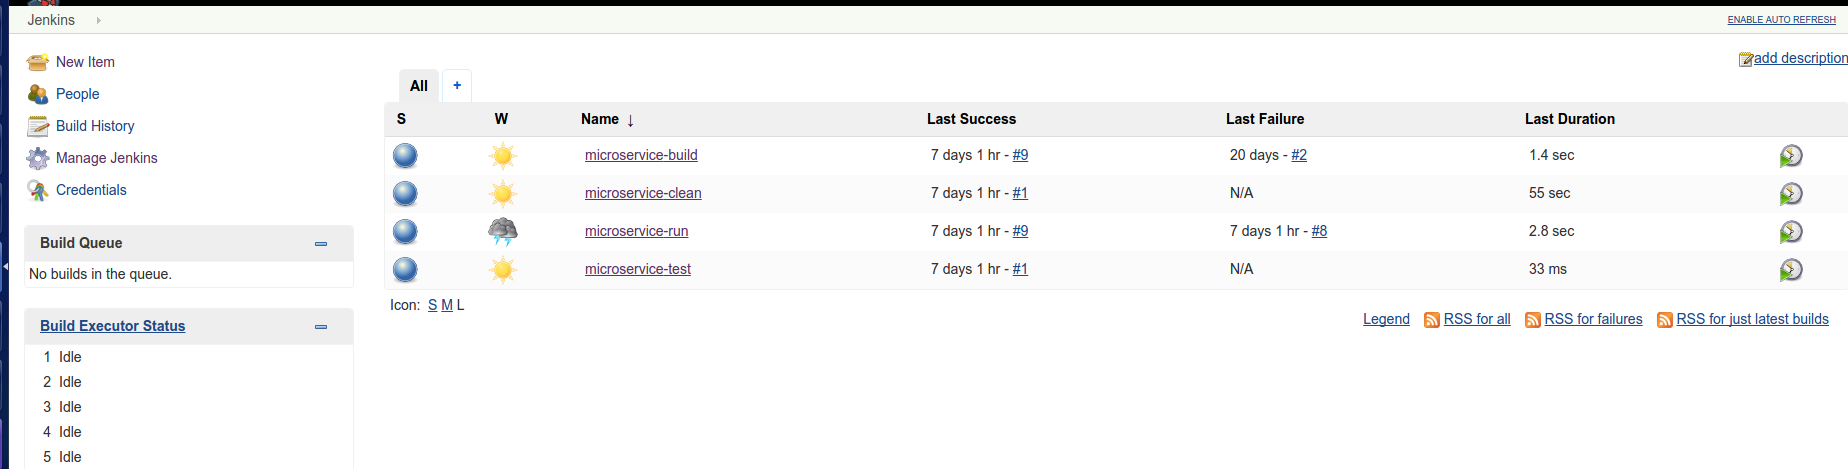
\includegraphics{img/jenkins-jobs.png}
\caption{Jenkins job-ok}
\end{figure}

\begin{itemize}
\tightlist
\item
  \textbf{bookstore-build}: Ennek a feladata a forrásfájlok és a Docker
  konténerek felkészítése. Miután a job végzett, a teljes infrastruktúra
  elkészíthető Docker konténerekből.
\end{itemize}

\begin{figure}[htbp]
\centering
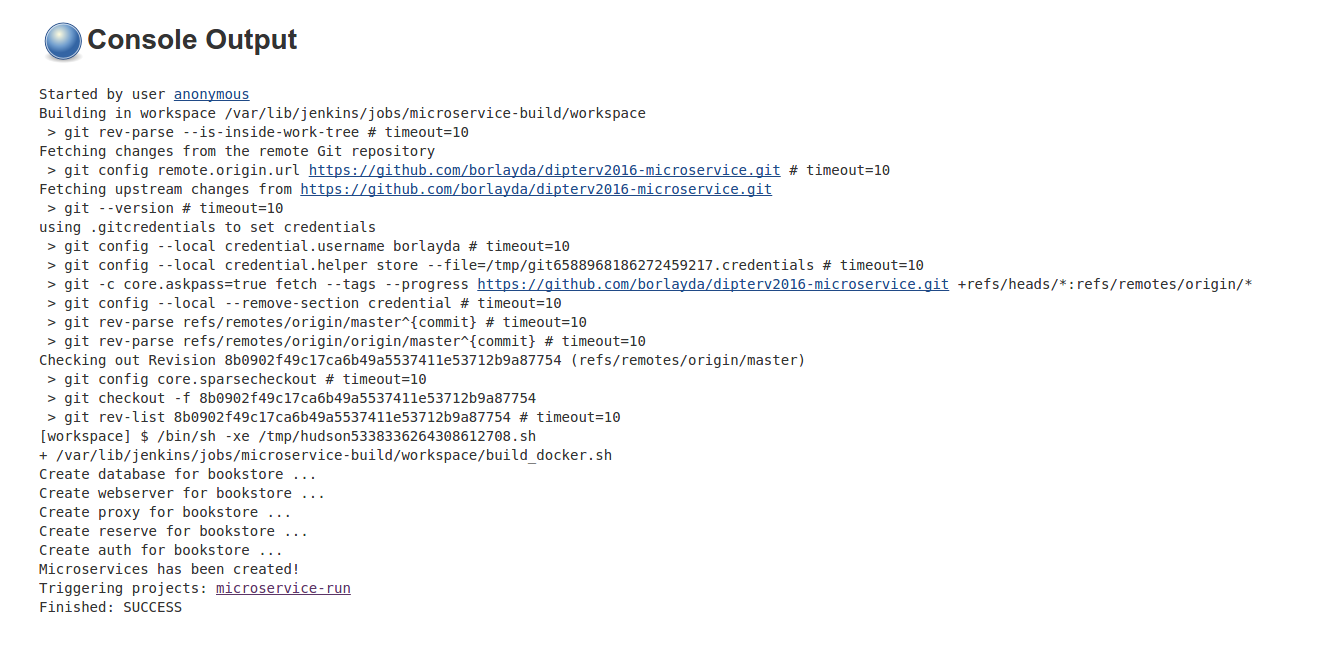
\includegraphics{img/jenkins-build.png}
\caption{Microservice build}
\end{figure}

\begin{itemize}
\tightlist
\item
  \textbf{bookstore-run}: Ennek a job-nak a feladata a Docker konténerek
  indítása, a szolgáltatások iniciaálizálása.
\end{itemize}

\begin{figure}[htbp]
\centering
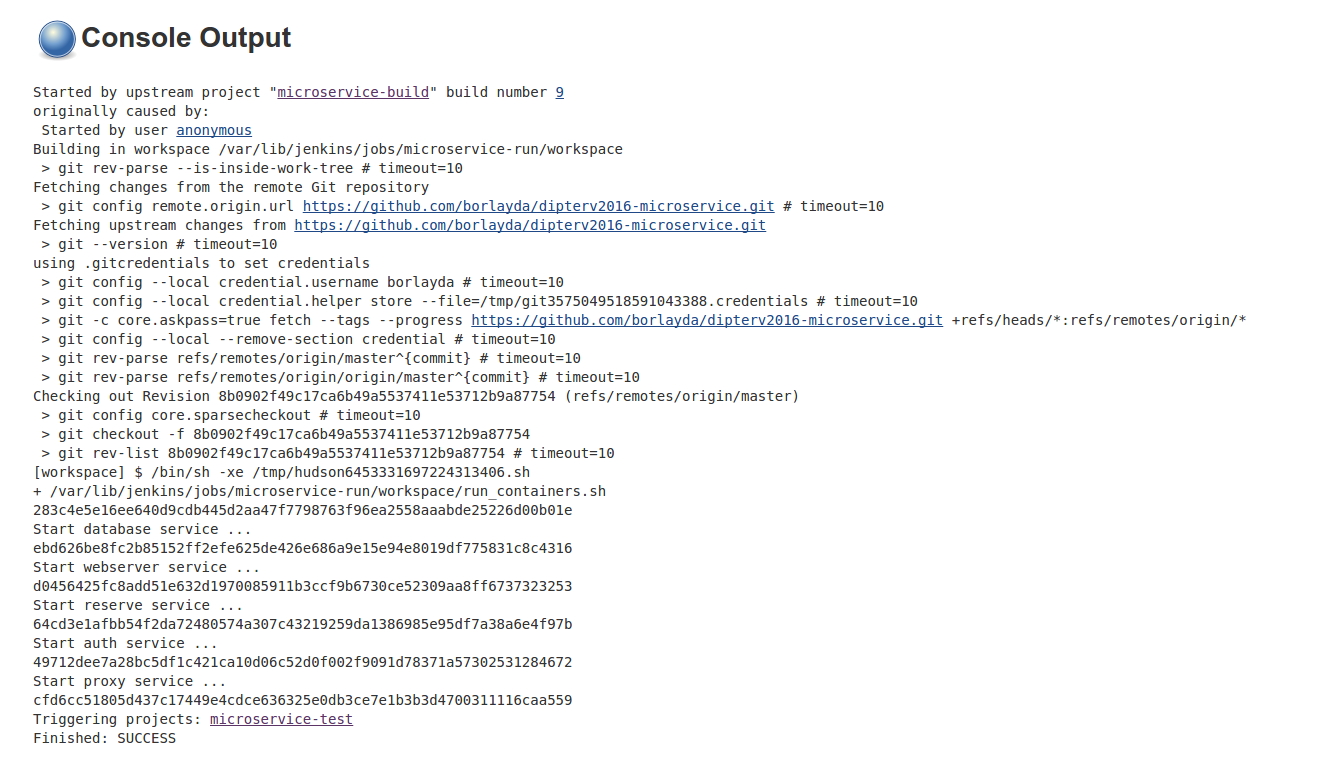
\includegraphics{img/jenkins-run.png}
\caption{Microservice run}
\end{figure}

\begin{itemize}
\tightlist
\item
  \textbf{bookstore-clean}: Ennek a job-nak a feladata, hogy a környezet
  ki legyen tisztítva, és ne maradjon a tesztek után semilyen Docker
  konténer, vagy fordított fájl a munkaterületen (workspace).
\end{itemize}

\begin{figure}[htbp]
\centering
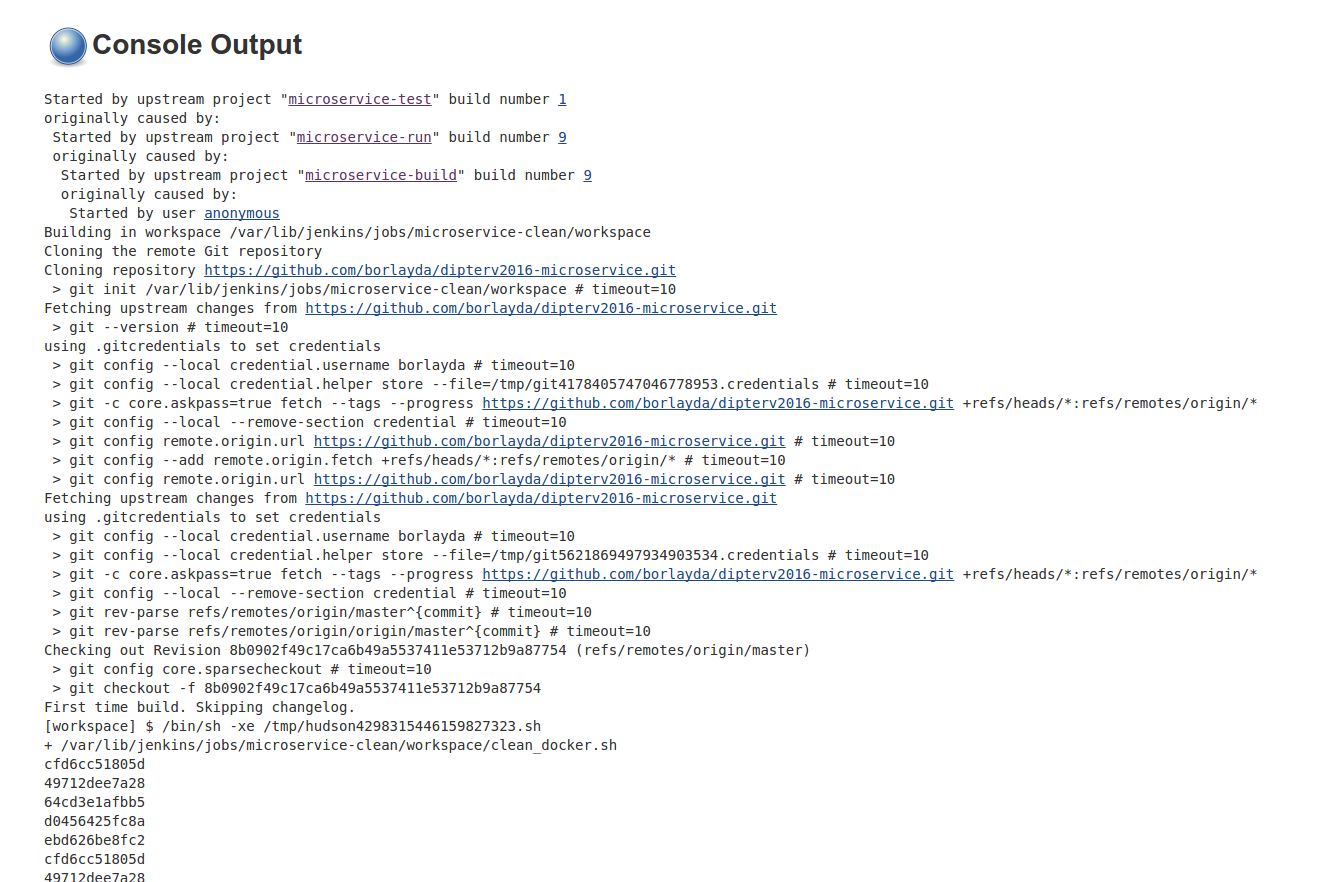
\includegraphics{img/jenkins-clean.png}
\caption{Microservice clean}
\end{figure}

\begin{itemize}
\tightlist
\item
  \textbf{bookstore-test}: Unit tesztek futtatása a feladata, de ide
  tartoznának a funkció és integrációs tesztek is, illetve a
  teljesítmény tesztek.
\end{itemize}

A Jenkins lehetővé teszi, hogy az egyes feladatok alfeladatokat
hívjanak, és egy komplex hierarchiát hozzanak létre. Ha bonyolultabb
vagy részletesebb felbontást szeretnék, csak fel kell vennem pár újabb
feladatot, és meg kell hívnom egy feladatból a többit.

\section{Egyéb minta
alkalmazások:}\label{egyuxe9b-minta-alkalmazuxe1sok}

KanBan board minta:

https://github.com/eventuate-examples/es-kanban-board

Archivematica minta:

https://www.archivematica.org/en/

\chapter{Összefoglaló}\label{uxf6sszefoglaluxf3}

A diplomaterv összefoglaló fejezete.

\chapter*{Irodalomjegyzék}\label{irodalomjegyzuxe9k}
\addcontentsline{toc}{chapter}{Irodalomjegyzék}

{[}7{]} Zohar Arad:
\href{http://zohararad.github.io/presentations/micro-services-monitoring/}{Effectively
Monitor Your Micro-Service Architectures}

{[}8{]} Nemeth Gergely:
\href{https://www.loggly.com/blog/monitoring-microservices-three-ways-to-overcome-the-biggest-challenges/}{Monitoring
Microservices}

{[}9{]} Cronitor:
\href{https://cronitor.io/help/micro-service-monitoring}{Monitoring
Microservices}

{[}10{]} Ruxit:
\href{https://ruxit.com/microservices/\#microservices_start}{Microservice
monitoring}

{[}11{]} Chris Richardson:
\href{http://microservices.io/patterns/service-registry.html}{Service
registry pattern}

{[}12{]} David Liu:
\href{https://github.com/Netflix/eureka/wiki/Eureka-at-a-glance}{Euraka
at glance}

{[}13{]} Hashicorp: \href{https://www.consul.io/}{Consul}

{[}14{]} Apache: \href{http://zookeeper.apache.org/}{Apache Zookeeper}

{[}15{]} Jenkins: \href{https://jenkins.io/index.html}{Jenkins}

{[}16{]} Netflix: \href{https://github.com/Netflix/eureka/wiki}{Eureka}

{[}17{]} Chef Software Inc.: \href{https://www.chef.io/chef/}{Chef}

{[}18{]} Ansible: \href{https://www.ansible.com/}{Ansible}

{[}19{]} SlatStack inc.: \href{http://saltstack.com/}{SaltStack}

{[}20{]} Amazon:
\href{https://aws.amazon.com/elasticloadbalancing/}{Elastic Load
Balancing}

{[}21{]} HAProxy: \href{http://www.haproxy.org/}{The Reliable, High
Performance TCP/HTTP Load Balancer}

{[}22{]} Fideloper LLC:
\href{https://serversforhackers.com/load-balancing-with-haproxy}{Load
Balancing with HAProxy}

{[}23{]} Nginx: \href{https://www.nginx.com/}{Nginx}

{[}24{]} Docker: \href{https://www.docker.com/}{Docker}

{[}25{]} Libvirt: \href{https://libvirt.org/}{libvirt: The
virtualization API}

{[}26{]} KVM: \href{http://www.linux-kvm.org/page/Main_Page}{Kernel
Virtual Machine}

{[}27{]} Zabbix: \href{http://www.zabbix.com/product.php}{What is
Zabbix}

{[}28{]} Elasticsearch:
\href{https://www.elastic.co/products/kibana}{Kibana}

{[}29{]} Elasticsearch:
\href{https://www.elastic.co/products/logstash}{LogStash}

{[}30{]} Cronitor.io: \href{https://cronitor.io/}{Cronitor}

{[}31{]} dynatrace:
\href{https://ruxit.com/why-ruxit/overview/\#whyruxitoverview_start}{Ruxit
overview}

\listoftables
\listoffigures

\bibliography{bibliography}


\appendix

\chapter{Függelék}\label{fuxfcggeluxe9k}

\end{document}
